\documentclass[11pt]{article}
%%%%%%%%%%%%%%%%%%%%%%%%%%%%%%%% Algunos Paquetes Necesarios 
\usepackage{fancyhdr, graphicx, wrapfig,lipsum}
\usepackage[utf8]{inputenc}% Language
\usepackage{pgf,tikz,pgfplots}
\usepackage[spanish]{babel}
\usepackage{xcolor}
\usepackage{mathrsfs}
\usetikzlibrary{arrows}
\pagestyle{empty}
\usepackage[margin=1in]{geometry} % Margins														
\usepackage{amssymb}
\usepackage{multicol}
\usepackage{amsmath, amsthm, amsfonts}
\usepackage{longtable} % Table accross multiple pages
\usepackage{hyperref}  % Use Hyperlinks
\usepackage{enumitem} % Reduce space in enumerate
\usepackage{txfonts}
\usepackage{float}
\usepackage{lipsum}
\usepackage{fancybox}
\usepackage[pangram]{blindtext}
\usepackage{tcolorbox}
\usepackage[framemethod=TikZ]{mdframed}
\usepackage{verbatim} 
\usepackage{listings}

\definecolor{codegreen}{rgb}{0,0.6,0}
\definecolor{codegray}{rgb}{0.5,0.5,0.5}
\definecolor{codepurple}{rgb}{0,0,1}
\definecolor{backcolour}{rgb}{0.9,0.9,0.9}

\lstdefinestyle{mystyle}{
	backgroundcolor=\color{blue!7},   
	commentstyle=\color{codegray},
	keywordstyle=\color{magenta},
	numberstyle=\tiny\color{codegreen},
	stringstyle=\color{codepurple},
	basicstyle=\ttfamily\footnotesize,
	breakatwhitespace=false,         
	breaklines=true,                 
	captionpos=b,                    
	keepspaces=true,                 
	numbers=left,                    
	numbersep=5pt,                  
	showspaces=false,                
	showstringspaces=false,
	showtabs=false,                  
	tabsize=2
}

\lstset{style=mystyle}





\begin{document}
	
	\newcommand{\myDoc}{Tarea 1.II.3}
	\newcommand{\myDate}{Primer semestre 2022}
	\newcommand{\myCourse}{Laboratorio Avanzado}
	\newcommand{\myName}{Rubí Esmeralda Ramírez Milián}
	\newcommand{\myCarnet}{201804565}
	\newcommand{\degre}{\ensuremath{^\circ}}
	\newcommand{\R}{\mathbb{R}}
	\newcommand{\F}{\mathbf{F}}
	\newcommand{\vi}{\mathbf{\hat{i}}}
	\newcommand{\vj}{\mathbf{\hat{j}}}
	\newcommand{\vk}{\mathbf{\hat{k}}}
	%%%%%%%%%%%%%%%%%%%%%%%%%%%%%%%%%%%%%%%Fancyboxes
	
	
	\newcounter{problem}[section]\setcounter{problem}{0}
	\renewcommand{\theproblem}{%\arabic{section}.
		\arabic{problem}}
	
	\newenvironment{problem}[1][]{%
		\refstepcounter{problem}
		
		\ifstrempty{#1}%
		% if condition (without title)
		{\mdfsetup{%
				frametitle={%
					\tikz[baseline=(current bounding box.east),outer sep=0pt]
					\node[anchor=east,rectangle,fill=purple!20]
					{\strut Inciso~\theproblem};}
			}%
			% else condition (with title)
		}{\mdfsetup{%
				frametitle={%
					\tikz[baseline=(current bounding box.east),outer sep=0pt]
					\node[anchor=east,rectangle,fill=purple!20]
					{\strut Inciso~\theproblem:~#1};}%
			}%
		}%
		% Both conditions
		\mdfsetup{%
			innertopmargin=10pt,linecolor=pink!40,%
			linewidth=2pt,topline=true,%
			frametitleaboveskip=\dimexpr-\ht\strutbox\relax%
		}
		\begin{mdframed}[]\relax%
			\label{#1}}{\end{mdframed}}
	
	
	\newcounter{solution}[section]\setcounter{solution}{0}
	\renewcommand{\thesolution}{%\arabic{section}.
		\arabic{solution}}
	\newenvironment{solution}[2][]{%
		\refstepcounter{solution}%
		\ifstrempty{#1}%
		{\mdfsetup{%
				frametitle={%
					\tikz[baseline=(current bounding box.east),outer sep=0pt]
					\node[anchor=east,rectangle,fill=green!20]
					{\strut Soluci\'on~\thesolution};}}
		}%
		{\mdfsetup{%
				frametitle={%
					\tikz[baseline=(current bounding box.east),outer sep=0pt]
					\node[anchor=east,rectangle,fill=green!20]
					{\strut Soluci\'on	~\thesolution:~#1};}}%
		}%
		\mdfsetup{innertopmargin=10pt,linecolor=green!20,%
			linewidth=2pt,topline=true,%
			frametitleaboveskip=\dimexpr-\ht\strutbox\relax
		}
		\begin{mdframed}[]\relax%
			\label{#2}}{\end{mdframed}}
	
	%%%%%%%%%%%%%%%%%%%%%%%%%%%%%%%%%%% Tema - BEGIN
	\newtheoremstyle{Tema}% name of the style to be used
	{5mm}% measure of space to leave above the theorem. E.g.: 3pt
	{3mm}% measure of space to leave below the theorem. E.g.: 3pt
	{}% name of font to use in the body of the theorem
	{}% measure of space to indent
	{\bfseries}% name of head font
	{\newline}% punctuation between head and body
	{20mm}% space after theorem head
	{}% Manually specify head
	
	\theoremstyle{Tema} \newtheorem{Tema}{Tema} %%%%% Template para Temas
	\theoremstyle{Tema} \newtheorem{serie}{Serie}              %%%%%  Template para Series de ejercicios
	\theoremstyle{Tema} \newtheorem{ejercicio}{Ejercicio}    %%%%%  Template para Ejercicios
	%%%%%%%%%%%%%%%%%%%%%%%%%%%%%%%%%%% Tema - END
	
	
	%%%%%%%%%%%%%%%%%%%%%%%%%%%%%%%%%%% Encabezado - BEGIN %%%%%%%%%%
	\fancypagestyle{firststyle}
	{
	
		\fancyhead[R]{
			\textbf{Universidad de San Carlos de Guatemala} \\
			\textbf{Escuela de Ciencias F\'isicas y Matem\'aticas}\\
			\textbf{\myName}\\
			\textbf{\myCourse }\\
			\textbf{\myCarnet}    %%%%%%%%%% Agregar nombre del curso 
			%%%%%%%%%%%%%%%%%%%%%% Agregar fecha en formato: Enero 15, 2015
		}
		\fancyhead[L]{ 
			%\includegraphics[height=1.6 cm, width=5.5 cm]{LogoColor}  
		}
	}
	%%%%%%%%%%%%%%%%%%%%%%%%%%%%%%%%%%% Encabezado - END %%%%%%%%%%
	
	%%%%%%%%%%%%%%%%%%%%%%%%%%%%%%%%%%% Encabezado (pagina 2 en adelante) - BEGIN %%%
	\fancypagestyle{allStyle}
	{
		\renewcommand{\headrulewidth}{1 pt}
		\fancyhead[R]{
			\emph{\myDoc $-$ \myCourse} %%%% Modificar n\'umero de examen parcial y nombre del curso
		}
		\fancyhead[L]{}  
		\fancyfoot[C]{}
		\fancyfoot[R]{\thepage}
	}
	%%%%%%%%%%%%%%%%%%%%%%%%%%%%%%%%%%% Encabezado (pagina 2 en adelante) - END %%%
	
	\date{}
	\setlength{\headheight}{0.65 in} % fixes \headheight warning
	%%%%%%%%%%%%%%%%%%%%%%%% BEGIN%%%%%%%%%%%%%%
	
	\pagestyle{allStyle}
	
	\thispagestyle{firststyle}
	%%%%%%%%%%%%%%%%%%%%%%%%%%%%%%%%% Titulo - BEGIN
	\begin{center}
		\LARGE
		\textsc{\myDoc}\\\normalsize % Modificar el N\'umero del examen parcial
		\medskip
		\hrule height 1pt
	\end{center}
	
\begin{problem}
	Utilizando la clase VecR2 como ejemplo, definir e implementar una	nueva clase llamada VecR3, que son vectores en $R^3$. Esta clase debe sobrecargar los siguientes operadores:
	
	\begin{itemize}
		\item operator+ para suma de dos vectores.
		\item  operator- para resta de dos vectores.
		\item operator- para negación de un vector.
		\item operator* para producto punto de dos vectores.
		\item operator* para multiplicar un vector por un flotante.
		\item operator/ para dividir un vector por un flotante.
		\item operator $\%$ para producto cruz de dos vectores.
		\item operator= para asignación.
		\item operator== para compraración de igualdad entre vectores.
		También se debe sobrecargar las siguientes funciones como amigas,		
		\item operator* para multiplicar un flotante por un vector.
		\item operator $\ll$ para desplegar el vector con cout.
		
 	\end{itemize}
		De la misma forma que en VecR2, se debe implementar un atributo estático que indique si al desplegar el vector, lo haga en forma cartesiana $(x, y, z)$ o esférica $(r, \theta, \phi )$.
\end{problem}

	Primero se debe hacer un archivo $ .hpp $ se encuentra en un repositorio, con el nombre \href{https://github.com/Mohs9/Lab-Avanzado/blob/eee254f75da3f1da0648a65ce5d045611bca5708/Tareas/T1_II_3/VecR3.hpp}{VecR3}
	
	
	En la cual, se ponen los atributos privados las coordenadas del vector y en modo público secrean los constructores y el destructoy además de todos los métodos, los primero son los métodos <<set>> y de <<get>>. 
	
	\begin{figure}[H]
		\centering
		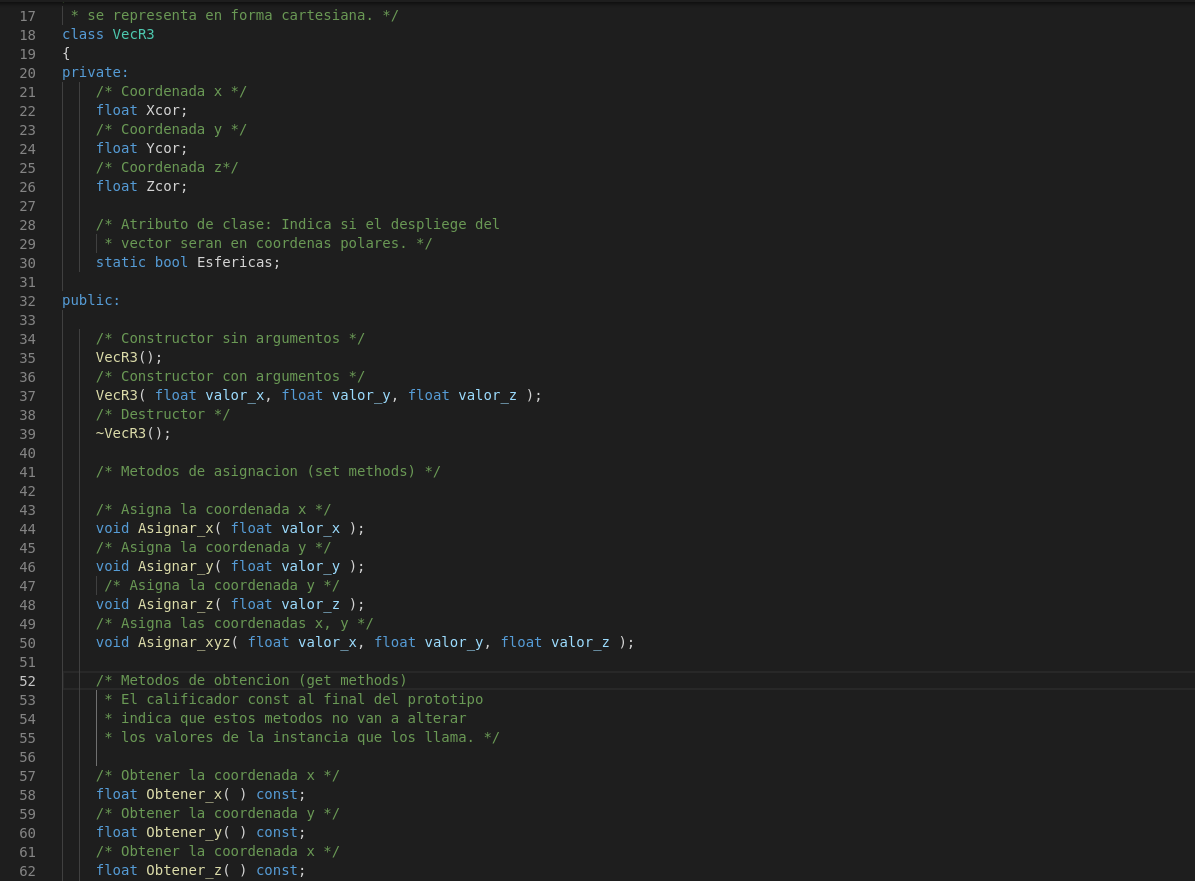
\includegraphics[width=0.7\linewidth]{img1}
		\caption{privado y público}
	\end{figure}
	
	
	Y la sobre carga de operadores, el operador magnitud devuelva un flotante, el operador de suma, de resta debuelven un vector, el operador * es el produto punto por lo que devuelve un flotante y los operadores de producto cruz y de asignación devuelven un vector y el operador de comparación devuelve un entero.
	
	\begin{figure}[H]
		\centering
		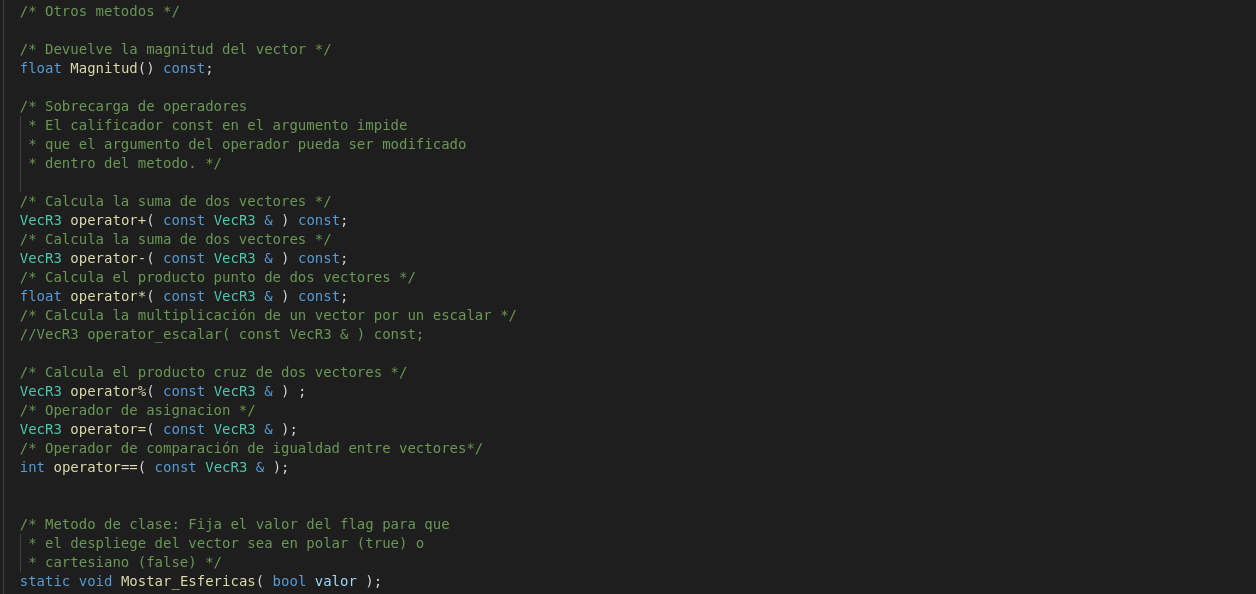
\includegraphics[width=0.7\linewidth]{img2}+
		\caption{sobrecarga de operadores}
	\end{figure}

	Y las funciones amigas que tienen acceso a los
	elementos privados en este caso a las coordenadas.
	
	
	\begin{figure}[H]
		\centering
		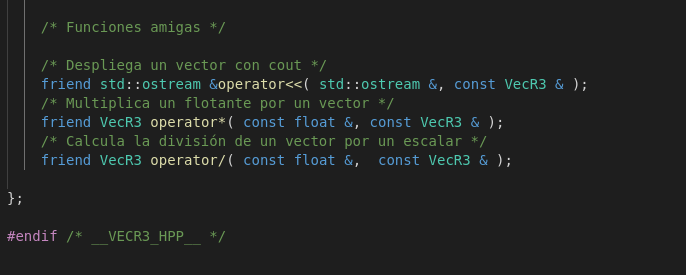
\includegraphics[width=0.7\linewidth]{img3}
		\caption{funciones amigas}
	\end{figure}
	
	Ahora se hace el archivo .cpp que se encuentra con el nombre \href{https://github.com/Mohs9/Lab-Avanzado/blob/eee254f75da3f1da0648a65ce5d045611bca5708/Tareas/T1_II_3/VecR3.cpp}{VecR3.cpp}
	
	\begin{figure}[H]
		\centering
		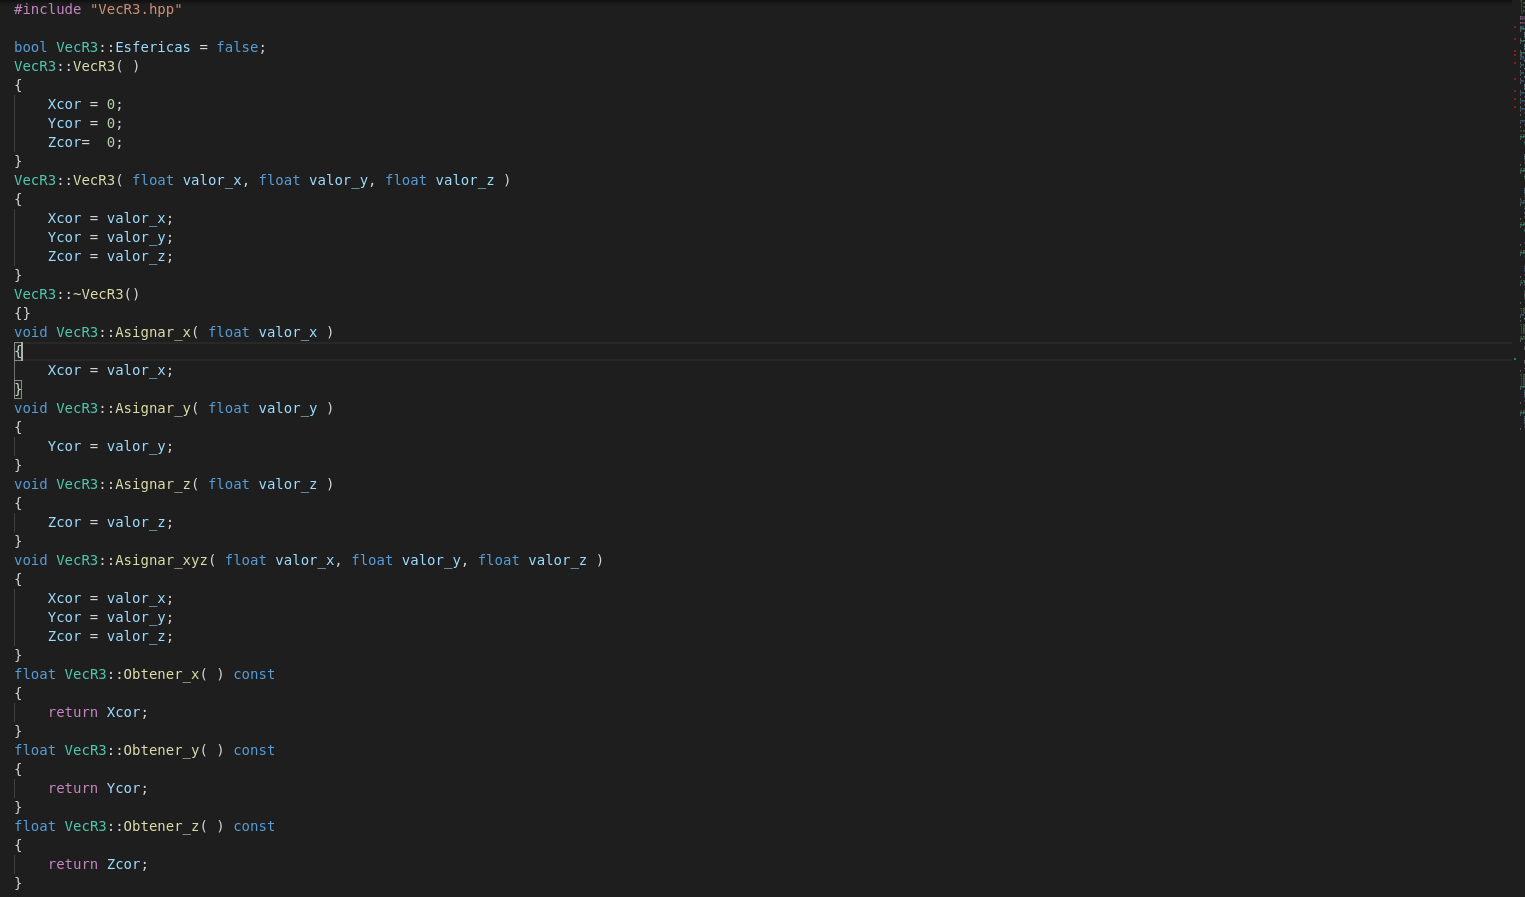
\includegraphics[width=0.7\linewidth]{img4}
		\caption{definir los primeros métodos. }
	\end{figure}
	
	
	
	Luego para la magnitd se utiliza la librería <<cmath>> para utilizar <<sqrt>>, Para sumar y restar vectores se debe utilizar dos vectores, uno de los vectores a restar o sumar es el que llama el operador, por lo que se accede a el por el puntero "this". El otro es el que se pasa como argumento. Como se esta dentro de las definiciones de clase, se puede acceder a los atributos privados.
	
	
	\begin{figure}[H]
		\centering
		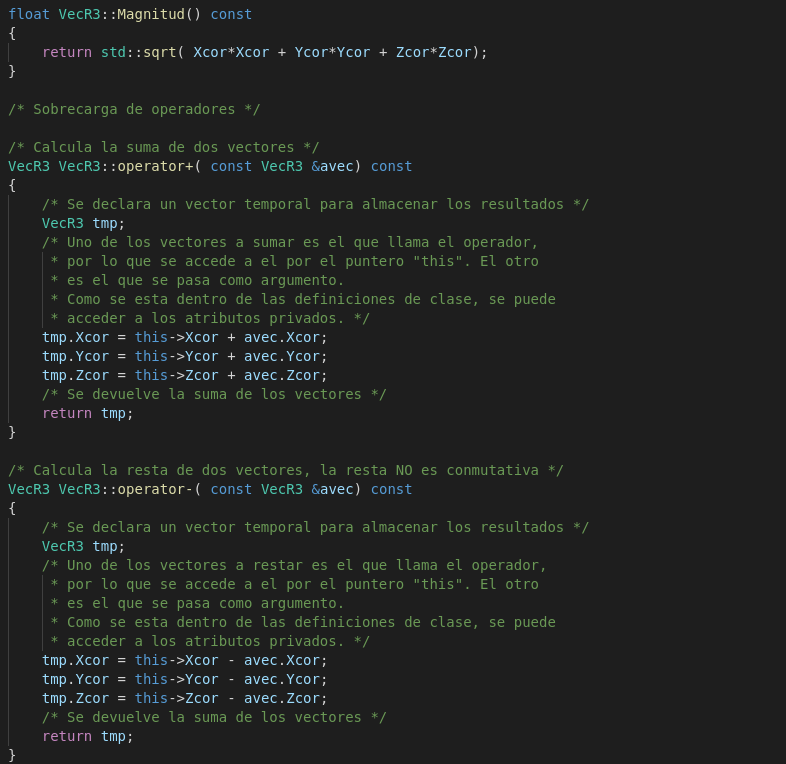
\includegraphics[width=0.7\linewidth]{img5}
		\caption{magnitud, operador suma y resta. }
	\end{figure}

	El operador del	producto interno también requiere dos vectores también pero devuelve un flotante. Y se multiplica coordenada a coordenada. Y el producto punto también utiliza el puntero this y se define coordenada a coordenada. Y el vector de asignación llama a otro vector y le asigna sus coordenadas al vector que lo llamó.
	
	\begin{figure}[H]
		\centering
		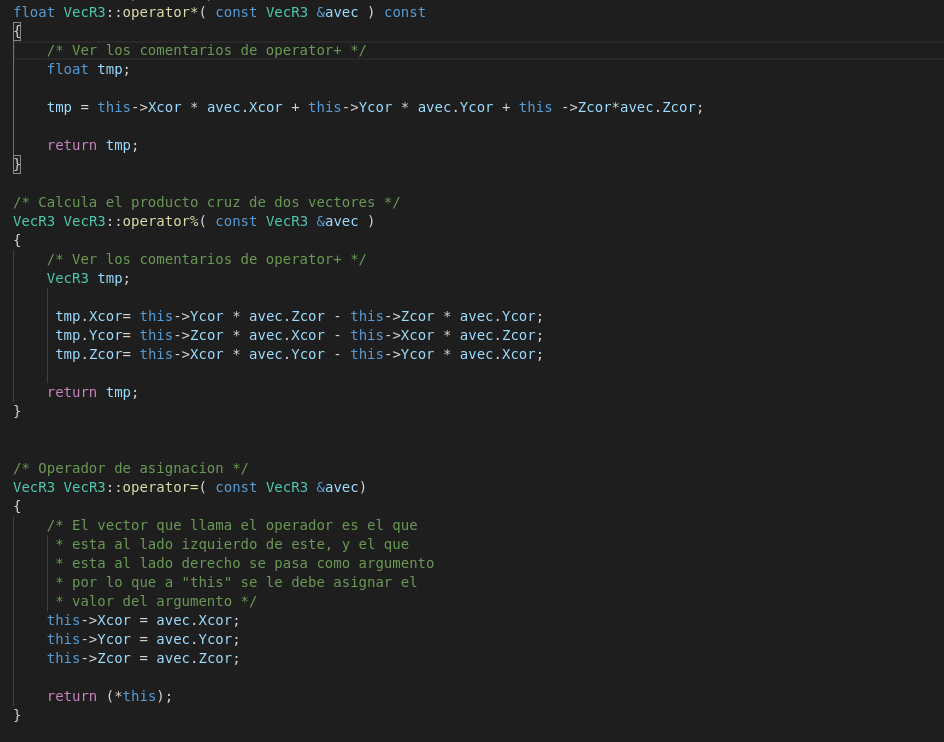
\includegraphics[width=0.7\linewidth]{img6}
		\caption{producto punto y producto cruz. }
	\end{figure}
	
	El operador de comparación analiza las coordenadas de ambos vectores y retorna un cero si son guales y uno si no son iguales, e imprime si son iguales o no.  El método de Mostrar\_Esfericas cambia el valor del flag "Esfericas". Y ostream pueden escribir secuencias de caracteres y representar otros tipos de datos. Se proporcionan miembros específicos para realizar estas operaciones de salida. Si el flag Esfericas es true el método Mostrar\_Esfericas muestra al vector en coordenadas esféricas.
	
	
	
	\begin{figure}[H]
		\centering
		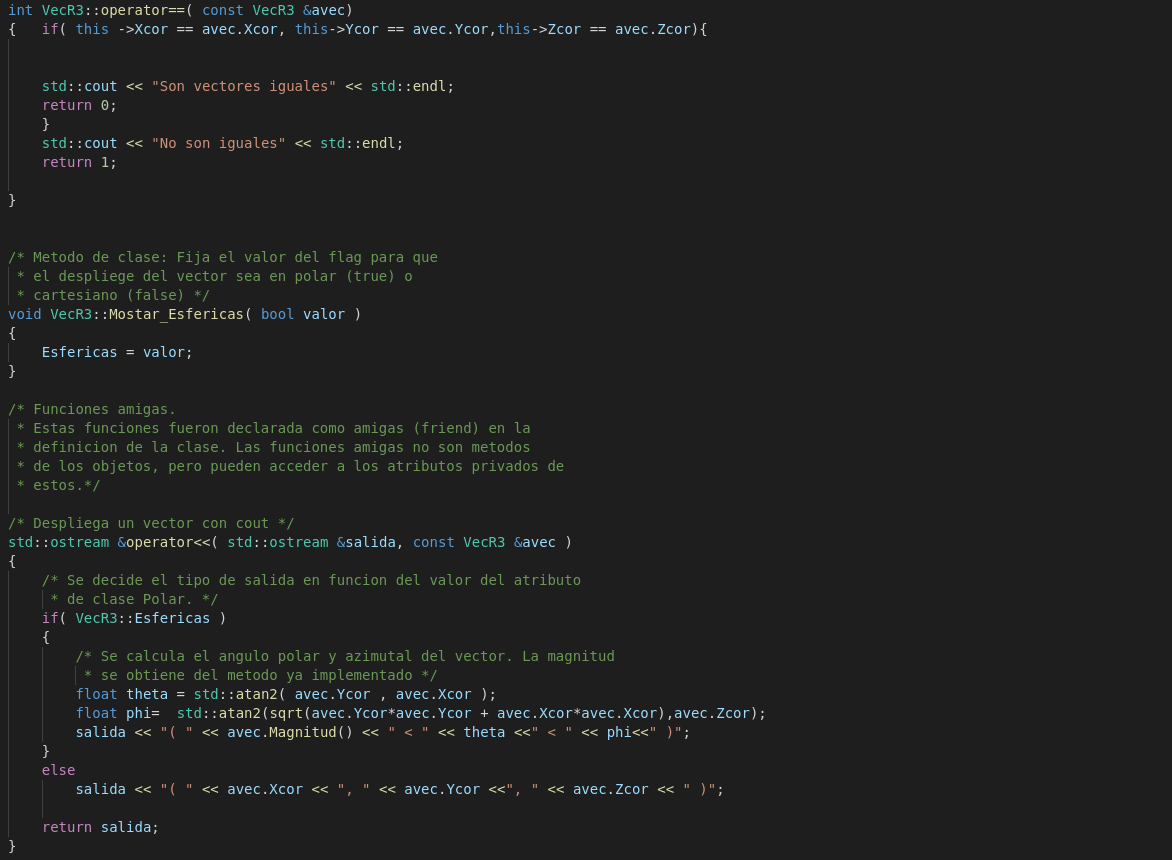
\includegraphics[width=0.7\linewidth]{img7}
		\caption{Otros operadores. }
	\end{figure}

Y por últimos se utiliza las funciones amigas que reciben un escalar y devuelven un vector, pueden acceder a los atributos privados.

	\begin{figure}[H]
	\centering
	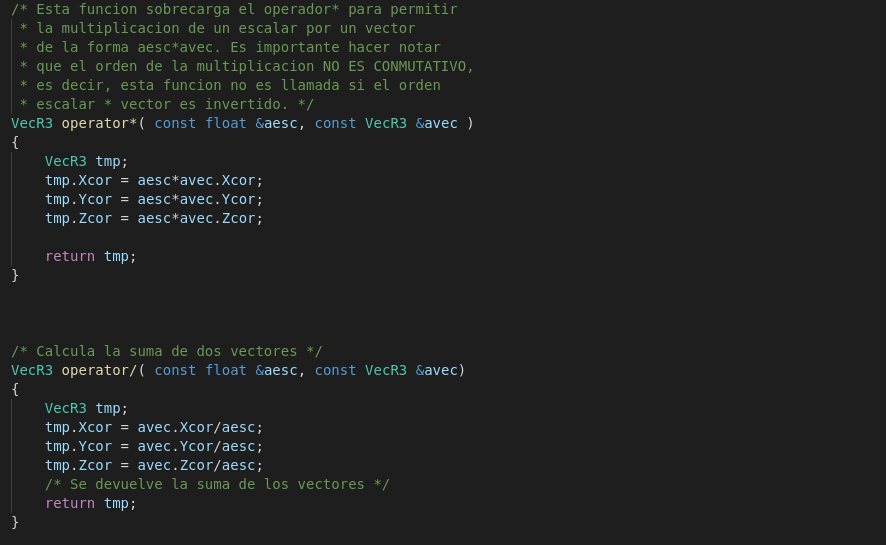
\includegraphics[width=0.7\linewidth]{img8}
	\caption{de nuevo funciones amigas. }
\end{figure}

Se comprueba el uso de estos operadores en otro archivo \href{https://github.com/Mohs9/Lab-Avanzado/blob/eee254f75da3f1da0648a65ce5d045611bca5708/Tareas/T1_II_3/prueba.cpp}{Prueba.cpp}, crean dos vecores y se imprime en consola las salidas de cada operador.


\begin{figure}[H]
	\centering
	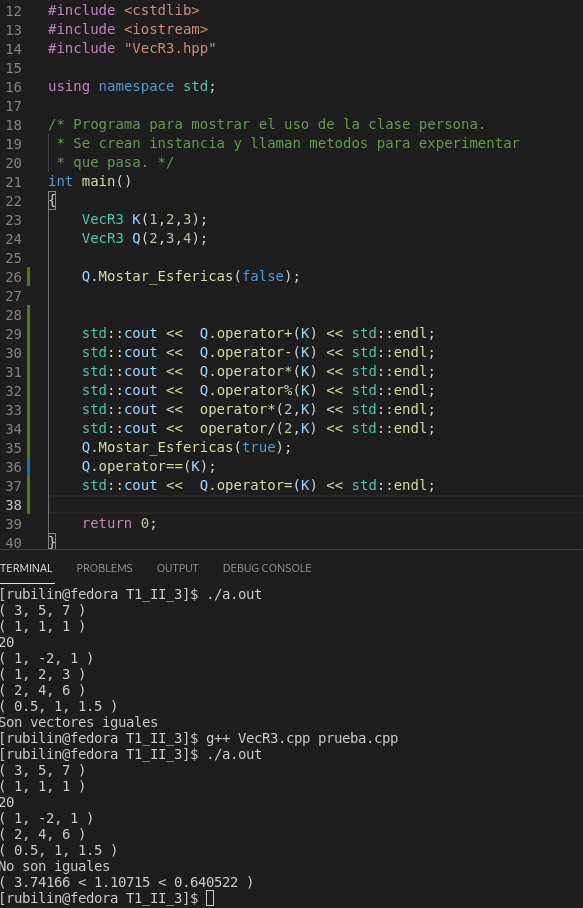
\includegraphics[width=0.4\linewidth]{img9}
	\caption{comprobación del funcioamiento de los operadores. }
\end{figure}






	
	%\bibliographystyle{ieeetr}% otras opciones {plain}
	%\bibliography{referencias}
	
	%%%%%%%%%%%%%%%%%%%%%%%%%%%%%%%%% Instrucciones - BEGIN
	
	\vspace{0.1 in}
	
\end{document} %%%%%%%%%%%%%%%%%%%%%%%% BEGIN%%%%%%%%%%%%%%